% !TeX root = ../../20260524.tex

\section{Applications}

\subsection{全排列}

\begin{frame}{例題一}
    \begin{problem}[TOJ 842 奇妙的排序]
        給一數 $N$

        問有多少個質數可以透過將 $N$ 的某些位數拿出來，任意排序後得到

        $1 \le N \le 10^6$
    \end{problem}
\end{frame}

\begin{frame}[fragile]{例題一解答}
    暴力把所有 $N$ 可以透過交換位數的數字枚舉出來

    那要怎麼枚舉?\pause

\begin{lstlisting}
next_permutation(a.begin(), a.end());
\end{lstlisting}

    一個 C++ 的語法，他會把 vector a 變成\textbf{下一個字典序的排列}，也會回傳有沒有這個排列
\end{frame}

\begin{frame}[fragile]{Code}
\begin{lstlisting}
string s; cin >> s;
sort(s.begin(), s.end());
do {
    int n = stoi(s);
    // do something
} while(next_permutation(s.begin(), s.end()));
\end{lstlisting}

時間複雜度為 $O(n!)$
\end{frame}

\subsection{枚舉子集合}

\begin{frame}{例題二}
    \begin{problem}[TOJ 656 枚舉子集和]
        有一個長度為 $n$ 的陣列 $A$

        計算有多少個子集合的和為 $k$

        $1 \le n \le 20$
    \end{problem}
\end{frame}

\begin{frame}{例題二解答}
    集合 $S = \{A_1, A_2, A_3, \ldots, A_n\}$

    要求的就是 $\sum_{T \subset S} [\sum_{a \in T} a = k]$\pause

    假如你有算過排列組合，那應該知道總共有 $2^{\lvert S \rvert}$ 個子集合

    為什麼呢?\pause

    每個元素有跟沒有，兩種狀態，總共 $\lvert S \rvert$ 個
\end{frame}

\begin{frame}[fragile]{例題二解答}
    枚舉子集合的方式也是一樣

    遞迴下去，每次遇到一個元素，就分岔出去兩種情況

\begin{lstlisting}
void dfs(int i, long long sum = 0) {
    if(i == n) { // 0 ~ n-1, n is the end
        if(sum == k) ans++;
        return;
    }
    dfs(i+1, sum); // 沒有
    dfs(i+1, sum+A[i]); // 有 Ai
}
\end{lstlisting}

時間複雜度為 $O(2^n)$
\end{frame}

\begin{frame}[fragile]{位元枚舉}
    枚舉方式也可以用位元枚舉

    我們用數字 $i$ 代表著集合 $T$ 的狀態

    假如數字 $i$ 的第 $j$ 位位元是 $1$ 就代表著集合 $T$ 有 $A_j$

\begin{lstlisting}
for(int i = 0; i < (1<<n); i++) {
    int sum = 0;
    for(int j = 0; j < n; j++) if(i&(1<<j)){
        sum += A[j];
    }
    if(sum == k) ans++;
}
\end{lstlisting}

時間複雜度 $O(2^n \cdot n)$，但常數很好
\end{frame}

\begin{frame}{題目}
    \begin{exercise}[CSES 1623 Apple Division]
        有 $n$ 個蘋果，每個有各自的重量 $p_i$

        將蘋果分成兩堆，使得兩堆的重量總和相差最小

        求相差最小可以是多少

        $1 \le n \le 20$

        $1 \le p_i \le 10^9$
    \end{exercise}
\end{frame}

\subsection{BFS 枚舉}

\begin{frame}{例題三}
    \begin{problem}[TOJ 429 D.巨人之杯]
        有 $3 \times 3$ 的拼圖，$1 \sim 8$ 然後少一格

        可以讓在空格四周的數字移動到空格上

        目標是讓他變成

        {
            \centering
            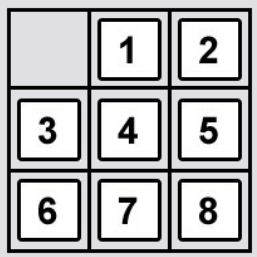
\includegraphics[width=3cm]{photos/TOJ-429.png}
        }

        $T$ 筆測資，輸出最少步數，假如無法達到，輸出 QQ

        $1 \le T \le 20$
    \end{problem}
\end{frame}

\begin{frame}{例題三解答}
    發現操作是將數字移動到空格上，發現這個操作是可逆的

    也就是說 開始狀態 $\to$ 到達狀態等於 到達狀態 $\to$ 開始狀態\pause

    考慮直接將開始狀態能到達的狀態枚舉出來，並記錄最短操作次數

    這樣就可以直接查表詢問了!

    那要怎麼暴力找所有狀態呢?\pause

    以後會介紹一個演算法叫做 BFS，可以做到剛剛所說的事情
\end{frame}